\documentclass[dvisvgm]{standalone}

\usepackage{amsmath}
\usepackage[usenames,dvipsnames]{xcolor}
\usepackage{tikz}
\usetikzlibrary {arrows.meta,
                 positioning,
                 shapes.geometric}

 \tikzset{
    square/.style={regular polygon, regular polygon sides=4},
        base/.style={draw, align=center, minimum height=4ex},
        proc/.style={base, rectangle, text width=8em},
        io/.style={trapezium, align=center, trapezium left angle=70, 
                   trapezium right angle=110, draw, text width=8em,
                   },
        test/.style={base, align=center, diamond, aspect=2,
                     %text width=5em
                     },
        term/.style={proc, rounded corners},
        myarrow/.style={-Stealth, line width=0.25mm},
 }

\begin{document}
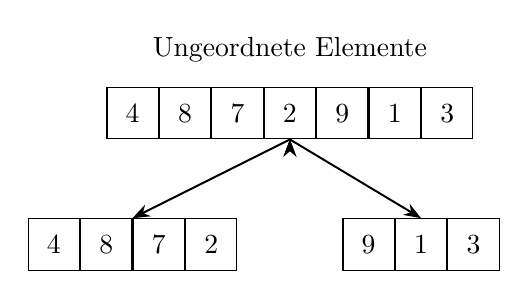
\begin{tikzpicture}
    \node[draw, square] (a) {4};
    \node[draw, square, right=0cm of a] (b) {8}; 
    \node[draw, square, right=0cm of b] (c) {7}; 
    \node[draw, square, right=0cm of c] (d) {2}; 
    \node[draw, square, right=0cm of d] (e) {9}; 
    \node[draw, square, right=0cm of e] (f) {1};
    \node[draw, square, right=0cm of f] (g) {3};  
    \node[above=2mm of d] (h) {Ungeordnete Elemente};

    \node[draw, square, below left=of d] (c2) {7};
    \node[draw, square, left=0cm of c2] (b2) {8};
    \node[draw, square, left=0cm of b2] (a2) {4};
    \node[draw, square, right=0cm of c2] (d2) {2};  

    \node[draw, square, below right=of d] (f2) {1};
    \node[draw, square, left=0cm of f2] (e2) {9};
    \node[draw, square, right=0cm of f2] (g2) {3};

    \draw[myarrow] (d.south) edge (c2.north west);
    \draw[myarrow] (d.south) edge (f2.north);

    

\end{tikzpicture}  
\end{document}